\documentclass[12pt]{article}
\usepackage{graphicx}
\usepackage{amsmath}
\usepackage{hyperref}
\usepackage{caption}
\usepackage{geometry}
\geometry{margin=1in}

\title{Optimization and Learning for Robot Control: Assignment 1}
\author{Luca Sartore - 256154}
\date{}


\begin{document}
\maketitle

\tableofcontents

\section{Test on Steady Robot}

\subsection{Q1: Baseline}

The baseline controller (the one with the default weights) shows decent tracking performance but is not perfect.
Errors on the center of mass along the $x$ and $z$ axes are minor (at most 1\,mm and 0.3\,mm, respectively), but the error along the $y$ axis (the one with the sine wave applied) is larger—about 3\,cm at the peak, as shown in Figure~\ref{fig:baseline}.

\begin{figure}[h!]
\centering
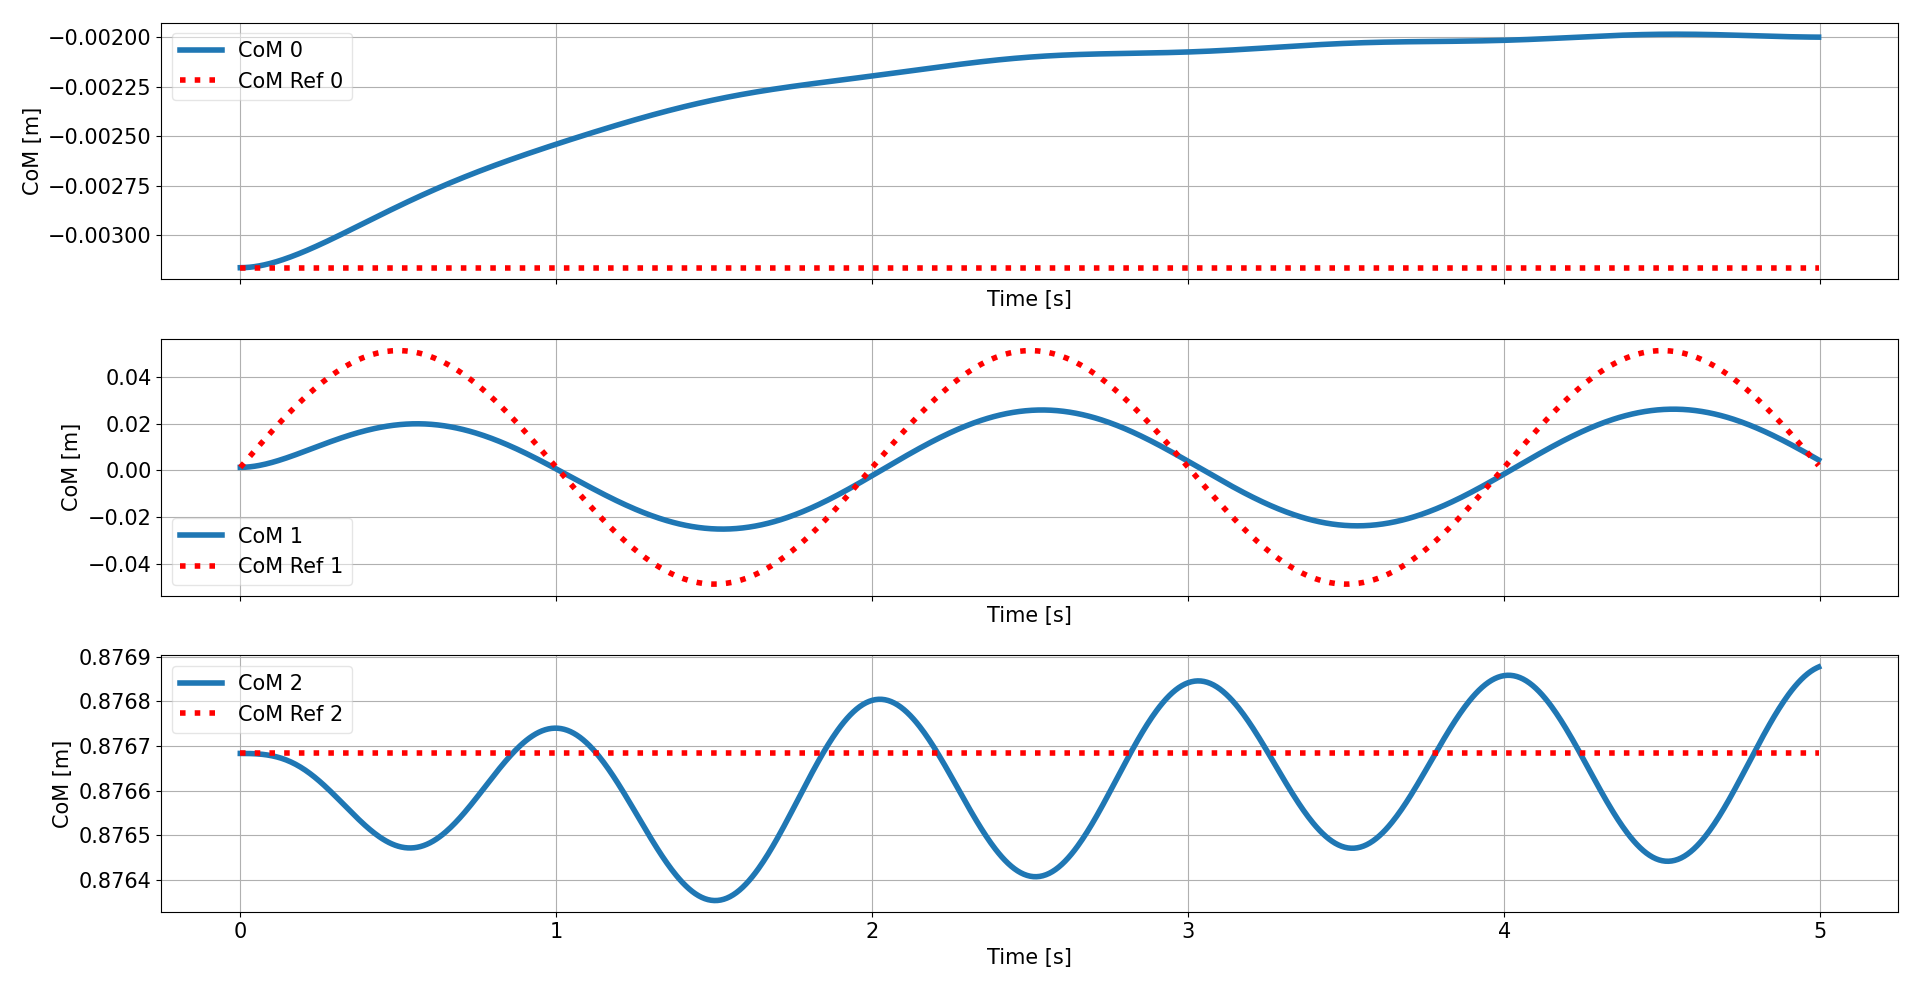
\includegraphics[width=0.6\textwidth]{./images/3.1.png}
\caption{Baseline controller performance.}
\label{fig:baseline}
\end{figure}

The most likely cause of the tracking error is that there are model inaccuracies resulting in unknown forces that are not compensated for by the controller.
Common sources of such errors include joint friction and damping.
Other possible causes are imprecise motor controllers or inaccuracies in the robot model (e.g., joint mass and inertia matrices).
However, since this experiment is conducted in simulation, these modeling errors should be minimal.

\subsection{Q2: Tuning the Parameters}

\subsubsection{Increasing the Weight of the Center of Mass Task}

In the first scenario (A), the weight of the center of mass task was increased from 1 to 10.  
The resulting performance is shown in Figure~\ref{fig:com_weight}.

\begin{figure}[h!]
\centering
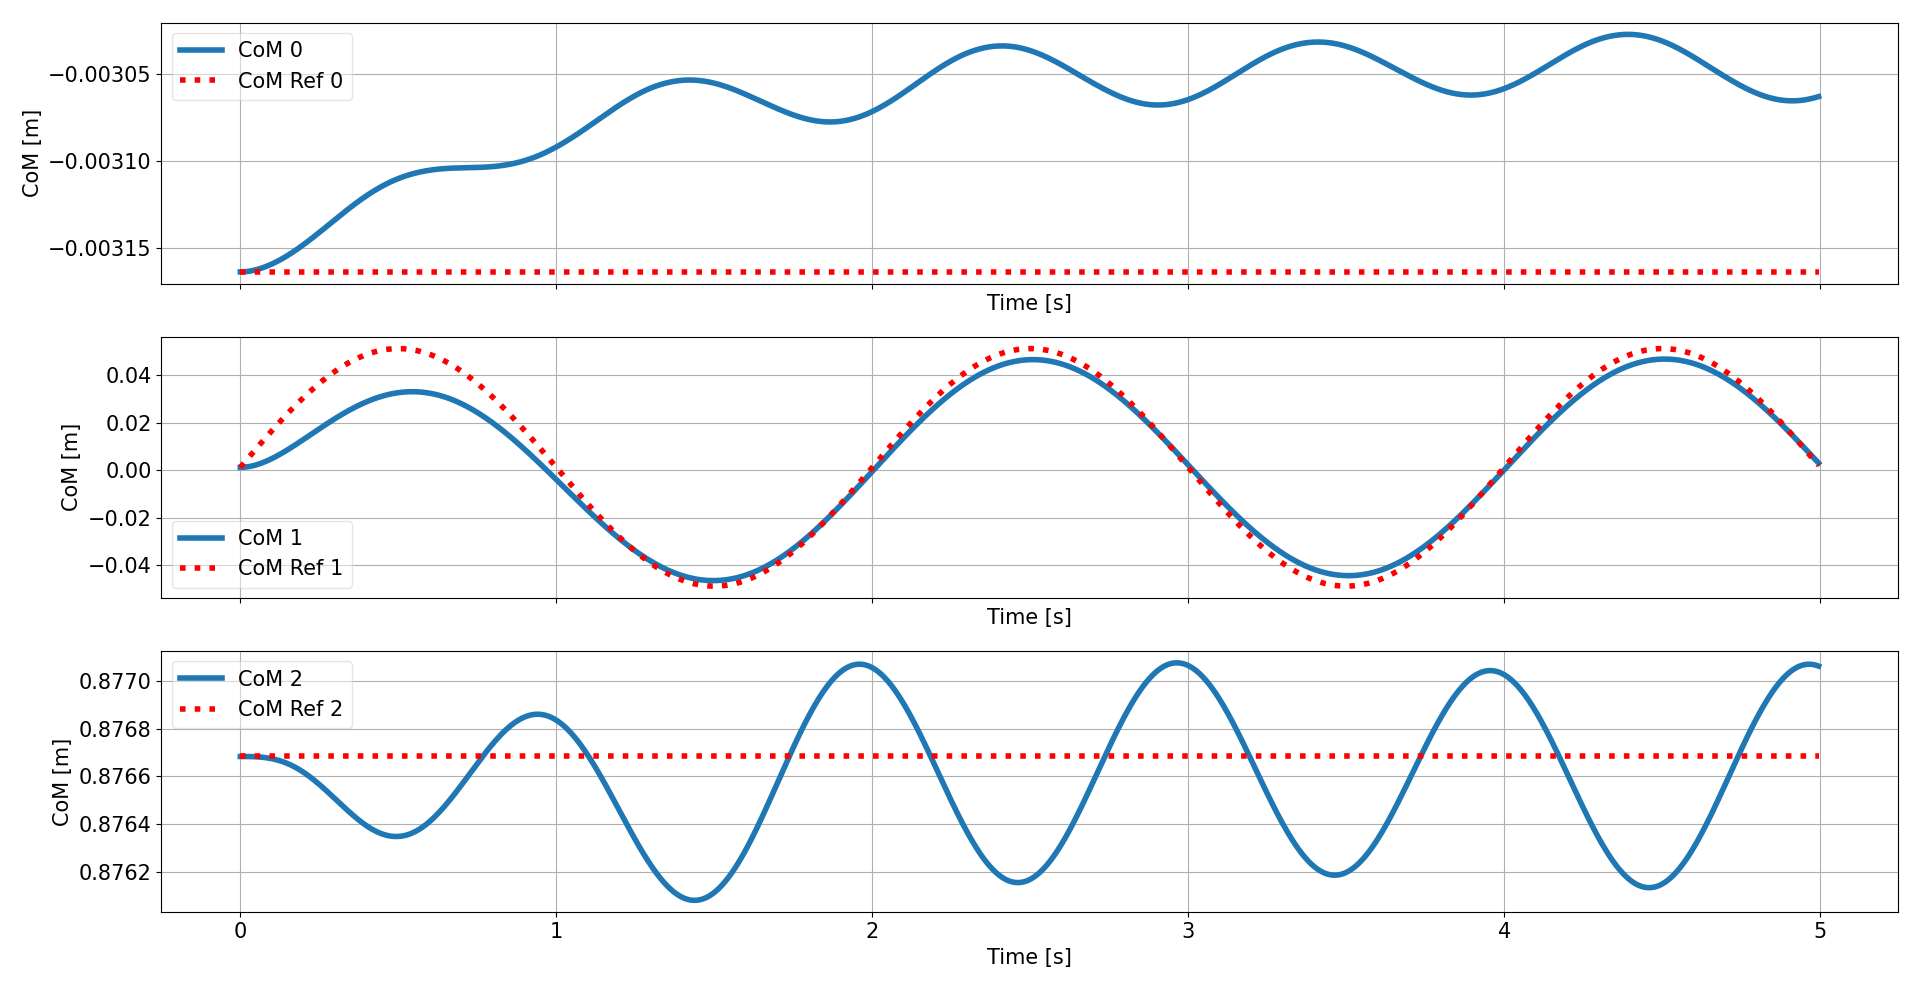
\includegraphics[width=0.6\textwidth]{./images/3.2.1.png}
\caption{Effect of increasing the center of mass task weight.}
\label{fig:com_weight}
\end{figure}

\subsubsection{Increasing the Proportional Coefficients of the Center of Mass Task}

In the second scenario (B), the proportional coefficient of the center of mass task was increased from 10 to 100.  
Results are shown in Figure~\ref{fig:com_gain}.

\begin{figure}[h!]
\centering
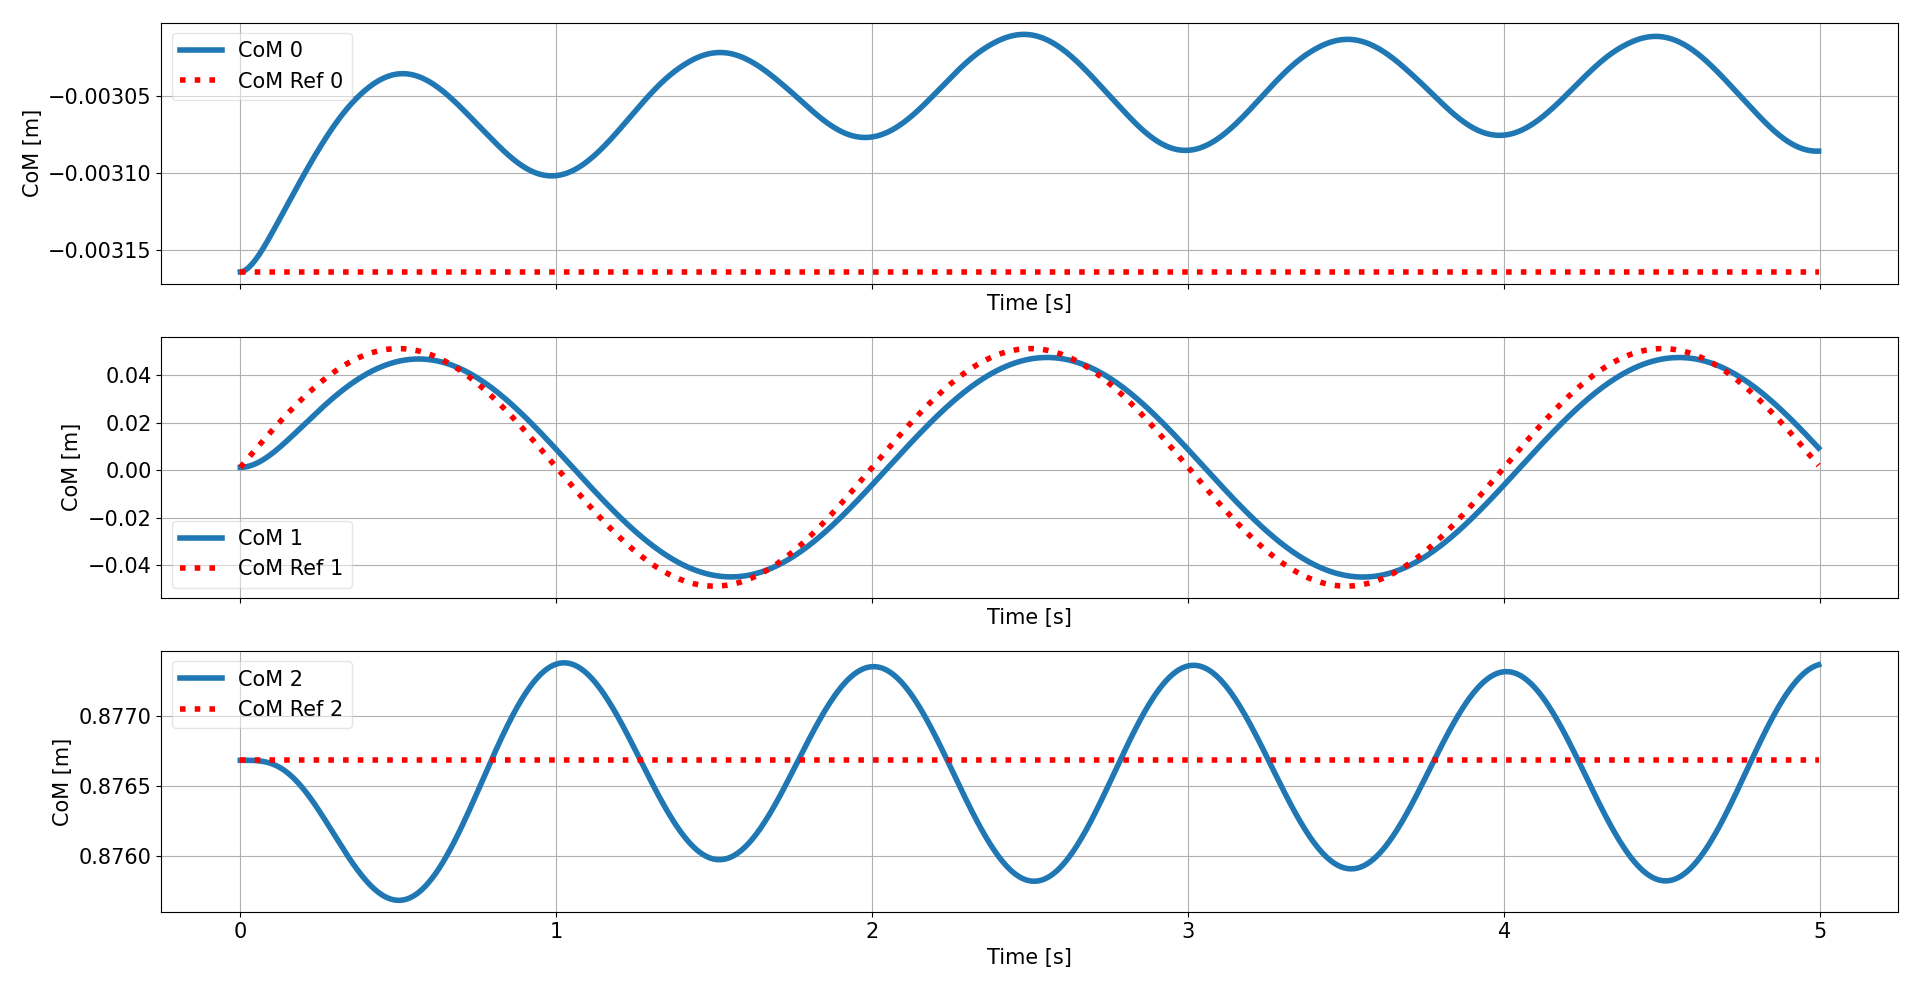
\includegraphics[width=0.6\textwidth]{./images/3.2.2.png}
\caption{Effect of increasing the proportional gain of the center of mass task.}
\label{fig:com_gain}
\end{figure}

\subsubsection{Differences Between the Two Scenarios}

\paragraph{Initial Behavior.}
Scenario A performs worse than scenario B at the beginning, showing a larger gap between the desired and actual positions.
We focus only on the $y$ axis (CoM1), since there are no significant differences along the other two axes.

\paragraph{Long-Term / Steady-State Behavior.}
After a few seconds, scenario A begins to perform better.  
The difference is minor, but scenario A keeps the actual trajectory closer to the desired one, while scenario B shows a small delay between the desired and actual trajectories.

The reason scenario A performs poorly initially is likely due to a weak control signal.  
As shown in Figure~\ref{fig:velocity}, the robot starts with zero velocity, yet an immediate “high” velocity is requested.
Controller B experiences a large initial error, which is multiplied by a high proportional gain, allowing it to reach the target more quickly.
Controller A, with a lower proportional gain, reacts more slowly.

\begin{figure}[h!]
\centering
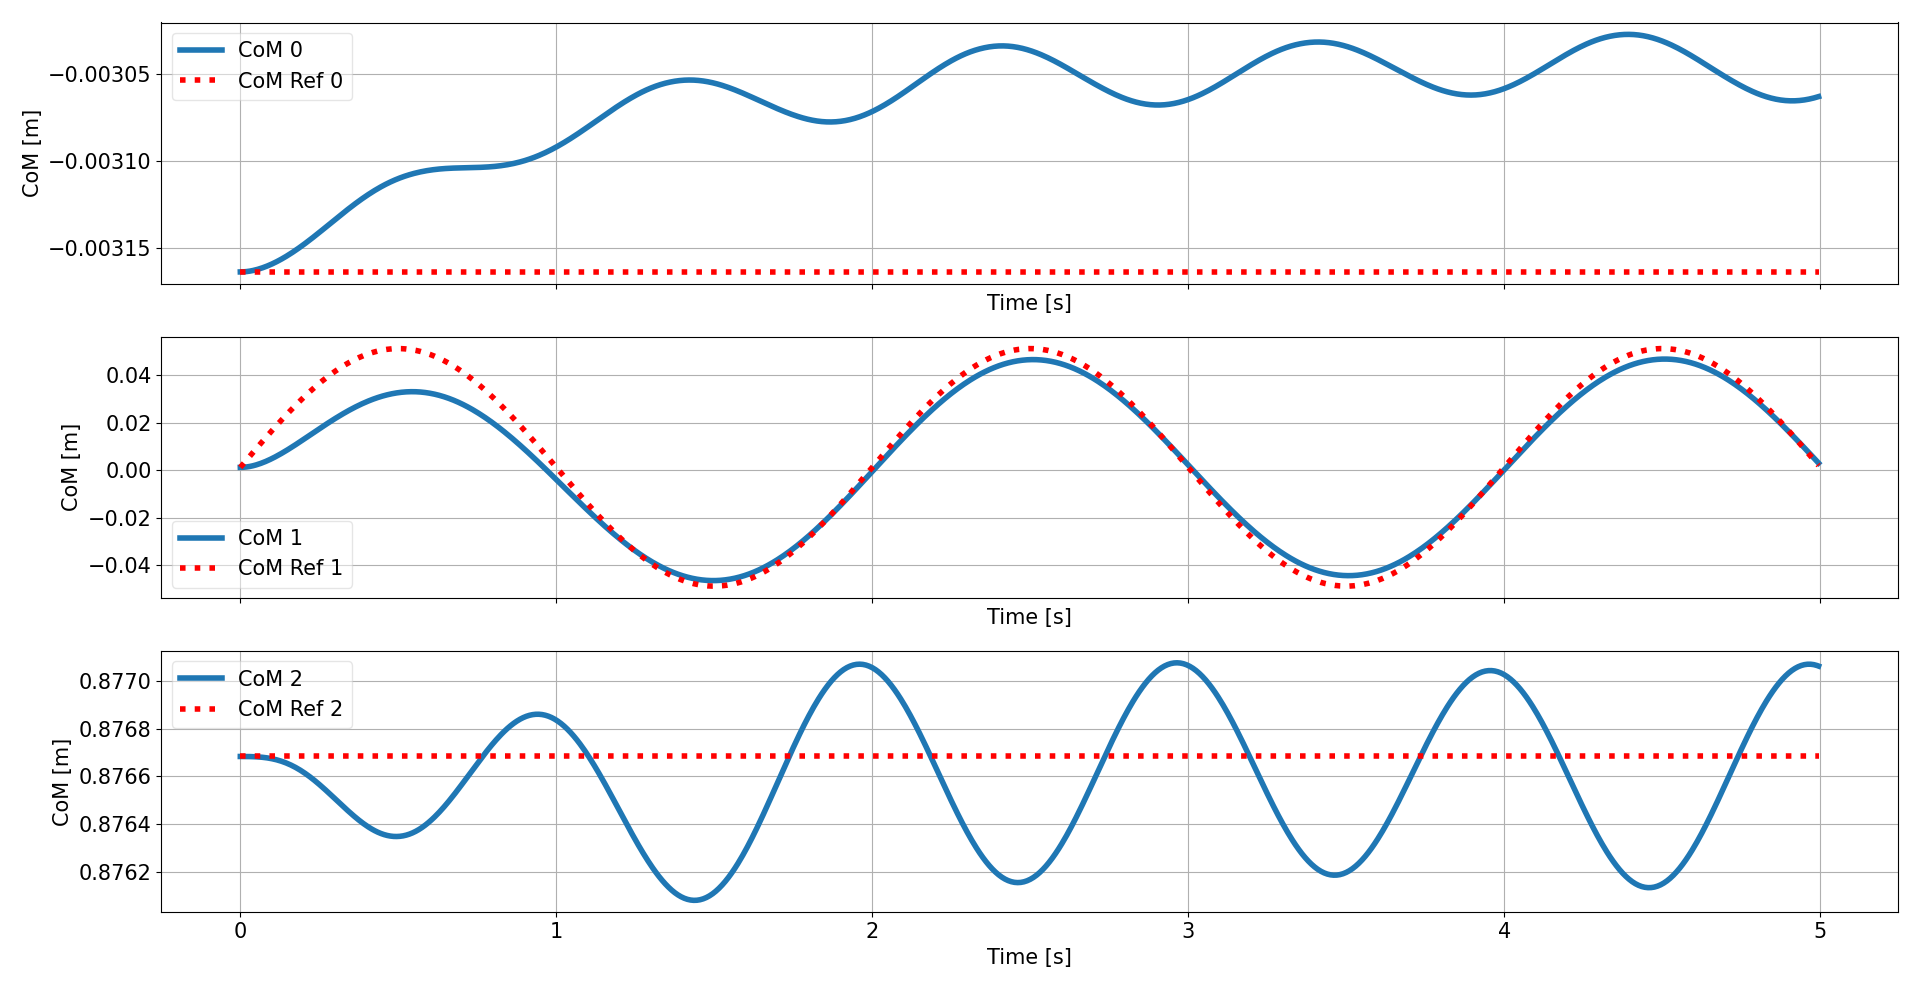
\includegraphics[width=0.6\textwidth]{./images/3.2.vel.png}
\caption{Velocity profiles}
\label{fig:velocity}
\end{figure}

In a real-world scenario, we would aim to provide a smoother control signal and start from zero velocity, in which case controller A would be preferred.
However, if sudden changes in velocity were common, controller B might perform better.

\subsection{Q3: Increasing Sine Wave Frequency}

In this third scenario, we increase the sine wave frequency to 1\,Hz and compare the two controllers (A and B).

\subsubsection{Controller A Performance}

Figure~\ref{fig:ctrlA} shows the center of mass tracking for controller A.  
Tracking performance is poor, and divergence between the desired and actual trajectories increases over time.

\begin{figure}[h!]
\centering
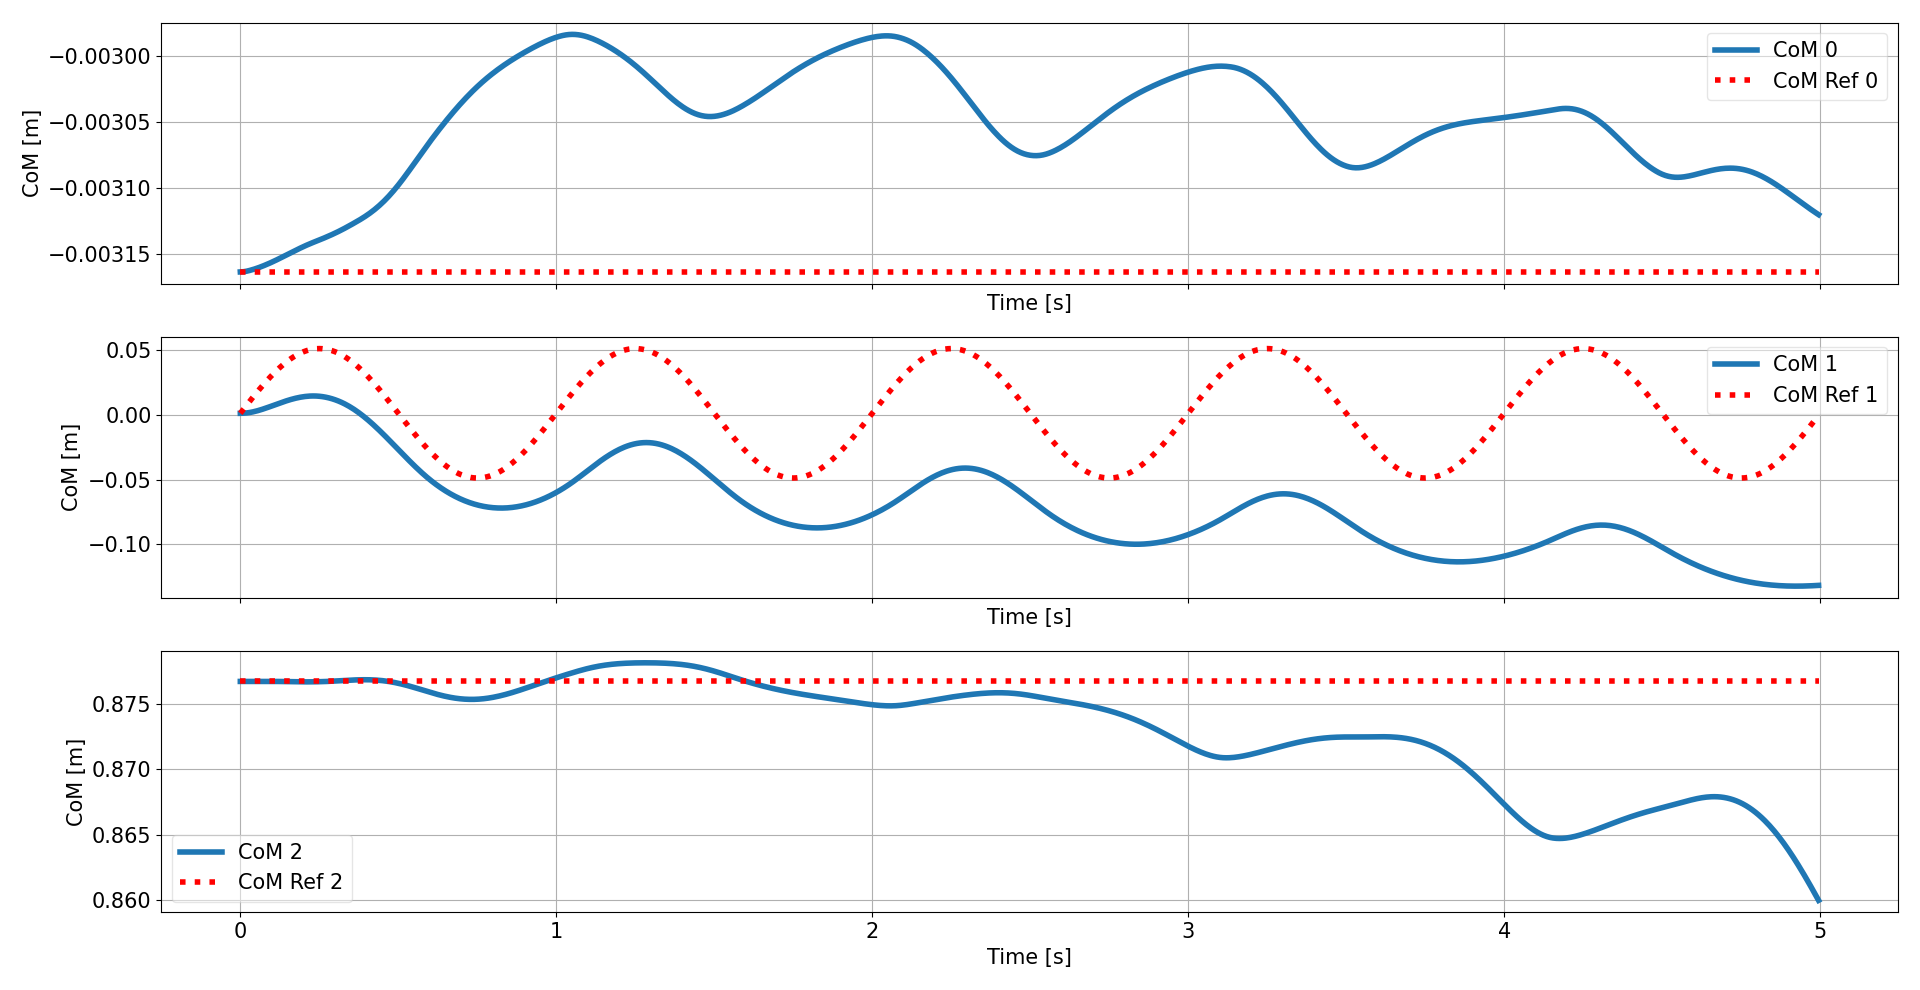
\includegraphics[width=0.6\textwidth]{./images/3.3.1.png}
\caption{Center of mass tracking for controller A at 1\,Hz.}
\label{fig:ctrlA}
\end{figure}

Examining the robot’s position at the final step (Figure~\ref{fig:ctrlA_robot}), we see that it is tilted sideways.  
This occurs because increasing the center of mass task weight decreases the relative importance of the postural task.  
The controller thus ignores maintaining an upright stance, leading to instability and poor tracking.  
Over time, the robot eventually collapses.

\begin{figure}[h!]
\centering
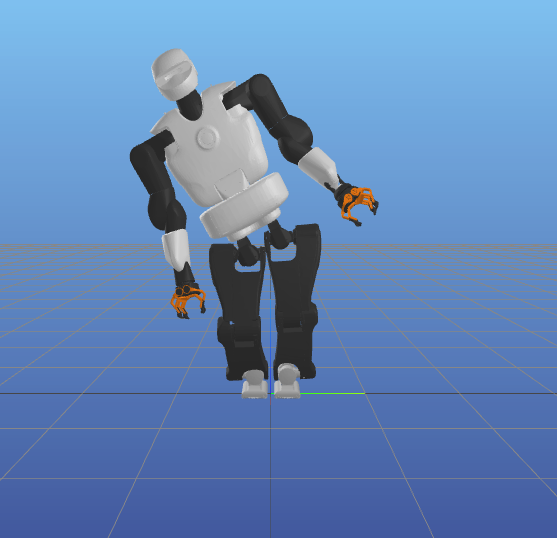
\includegraphics[width=0.5\textwidth]{./images/3.3.1.robot.png}
\caption{Robot posture for controller A at the final step.}
\label{fig:ctrlA_robot}
\end{figure}

In this case, controller B would clearly be preferred.

\subsubsection{Controller B Performance}

Controller B also performs poorly, as shown in Figure~\ref{fig:ctrlB}.  
The difference between desired and actual trajectories is larger compared to the lower-frequency test.
This is expected, since increasing the sine wave frequency increases the required velocity, which in turn demands higher torques.  
If the proportional coefficient remains constant, a higher error is required to produce the necessary torques.

\begin{figure}[h!]
\centering
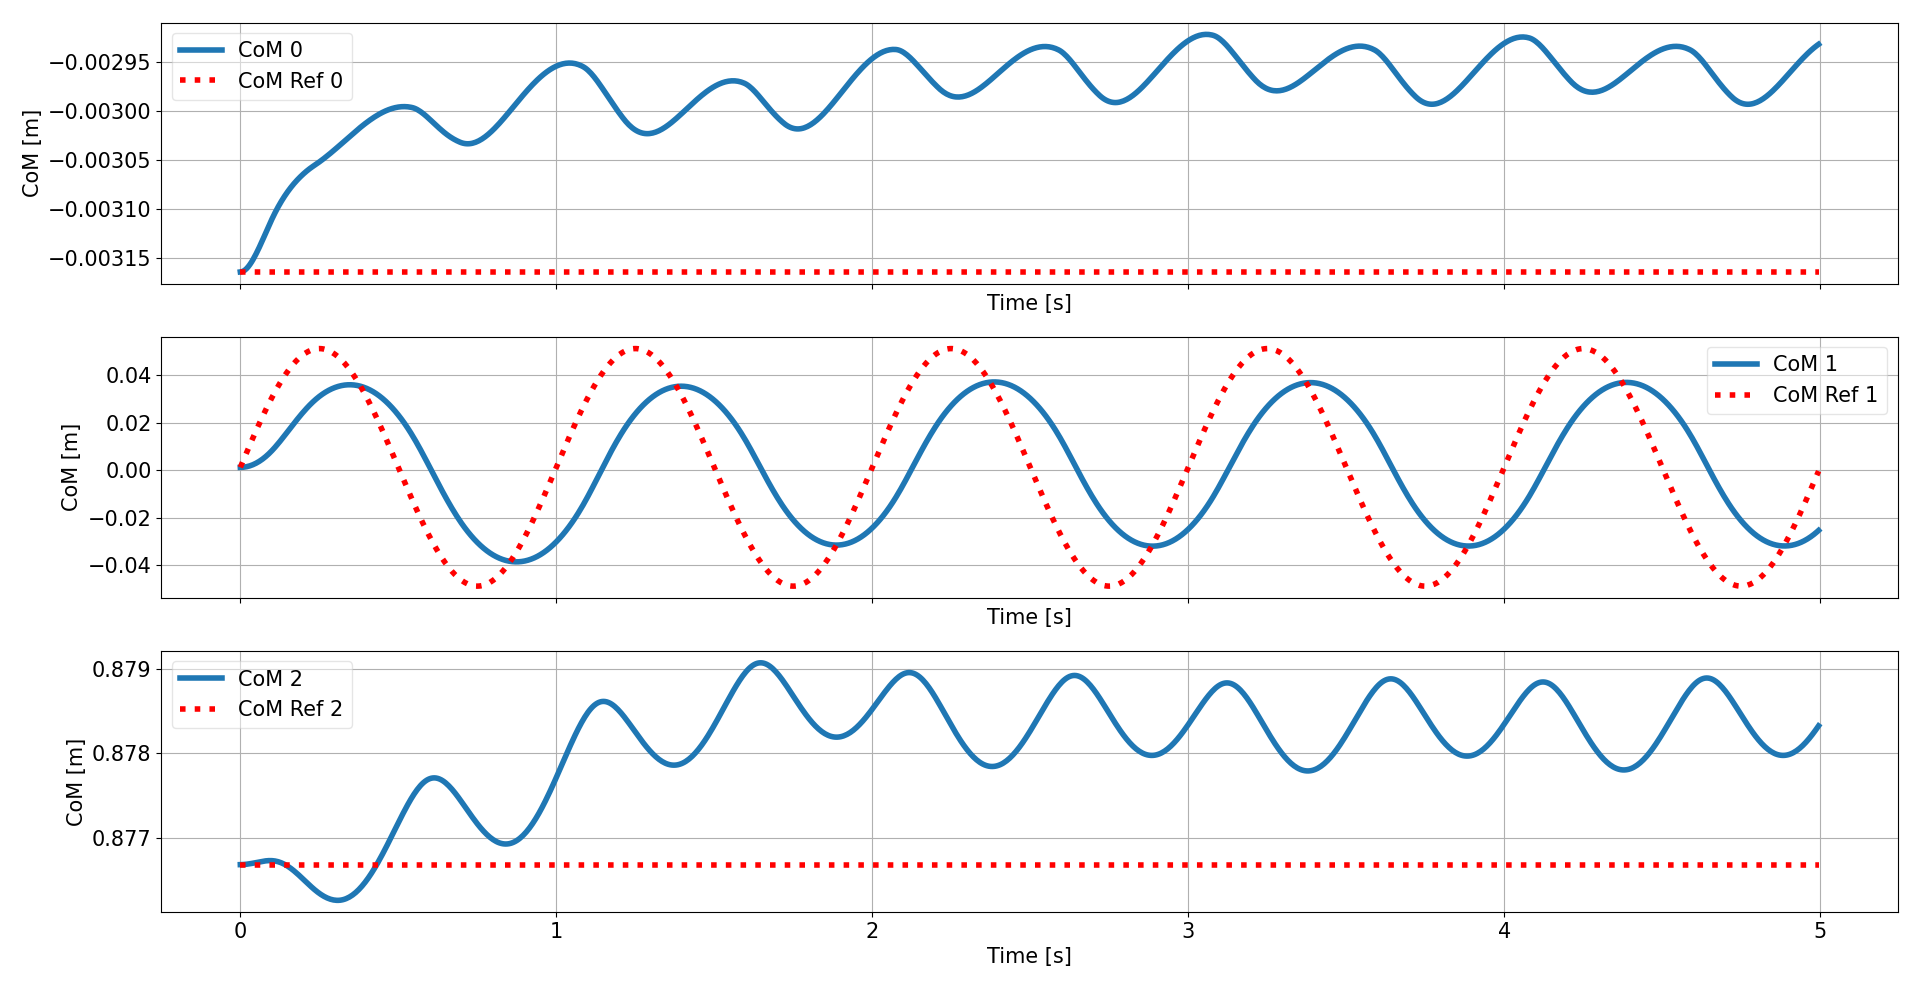
\includegraphics[width=0.6\textwidth]{./images/3.3.2.png}
\caption{Controller B tracking performance at 1\,Hz.}
\label{fig:ctrlB}
\end{figure}

\section{Test on Walking Robot}

\subsection{Q1: Experiment on 15\,cm Steps}

\subsubsection{Tuning the Postural Task Weight}

Initially, the robot was unable to stay upright and tilted sideways before falling—similar to controller A in the previous tests.
Increasing the postural task weight from zero to somewhere between $10^{-2}$ and $10^{-3}$ stabilized the robot.
A final value of $10^{-3}$ produced the tracking shown in Figure~\ref{fig:walking15}, which demonstrates excellent performance.

\begin{figure}[h!]
\centering
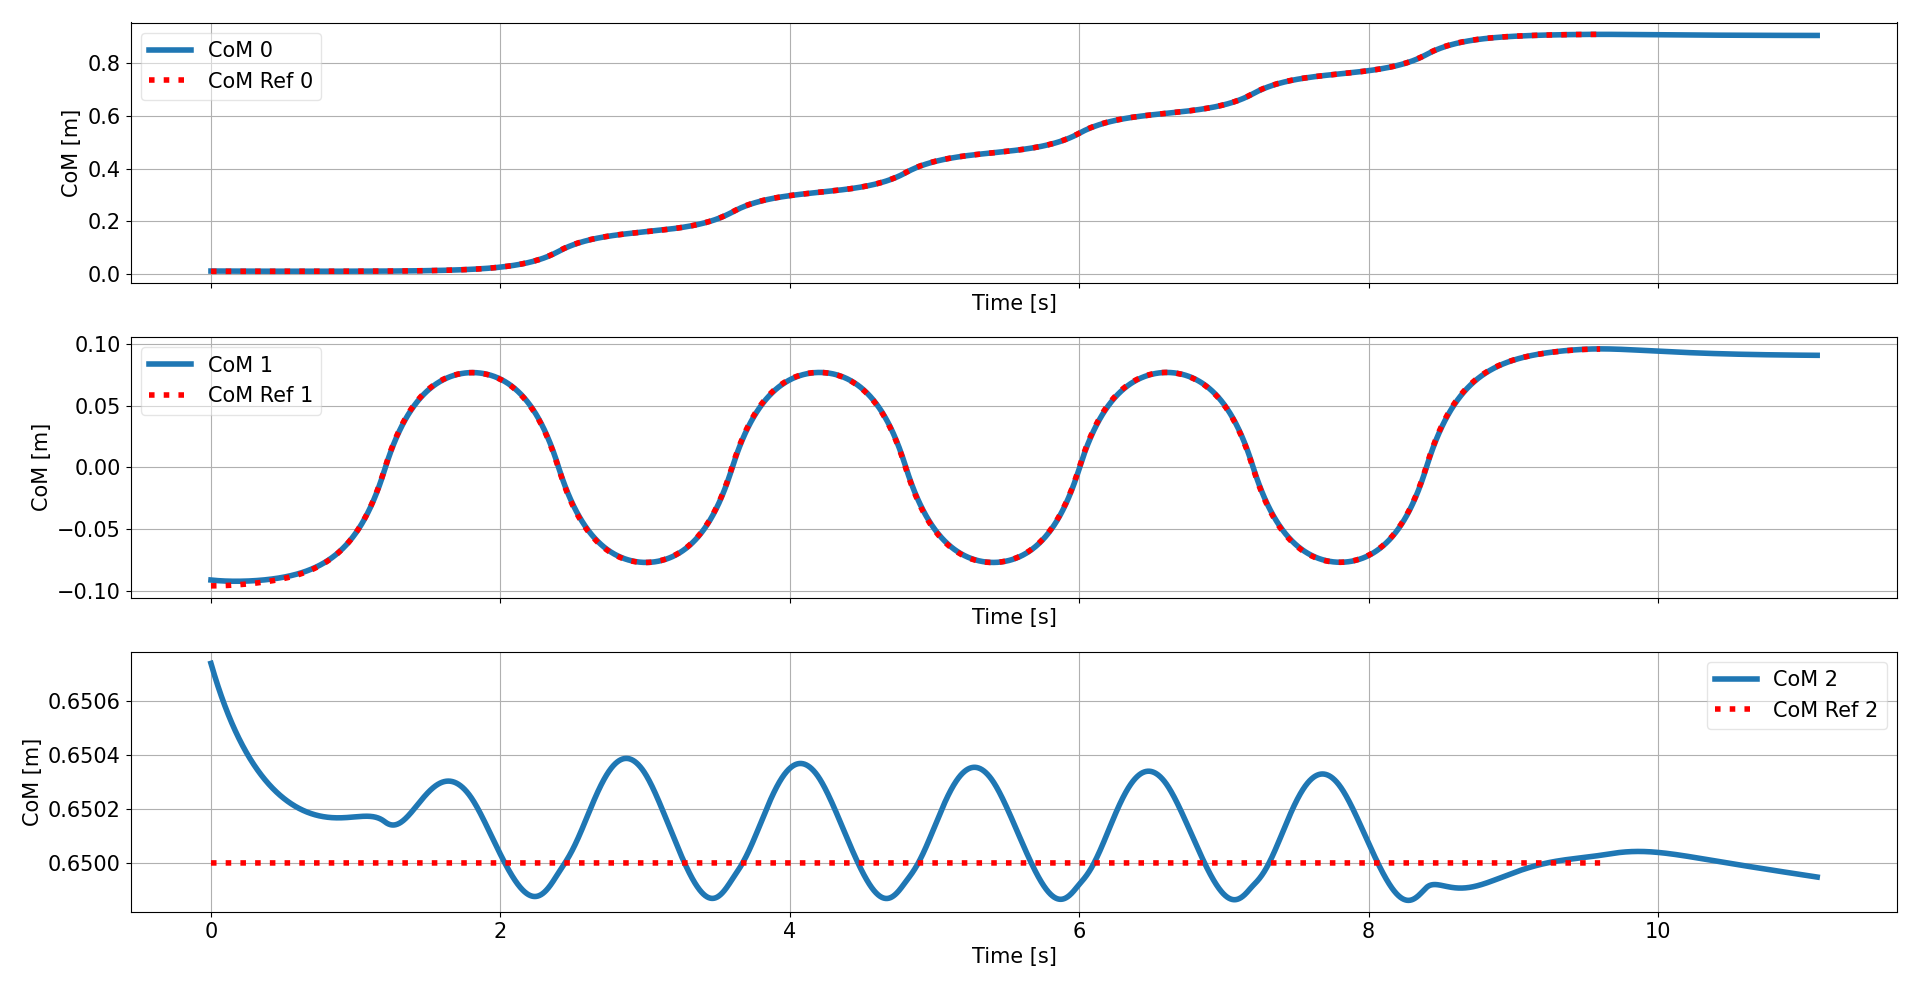
\includegraphics[width=0.6\textwidth]{./images/4.1.png}
\caption{Tracking performance for walking robot with 15\,cm steps.}
\label{fig:walking15}
\end{figure}

\subsubsection{Effect of Different Tasks on Robot Behavior}

To evaluate the effect of each task on walking performance, each task weight was set to zero individually, and the resulting behavior was observed.

\paragraph{Center of Mass Task.}
When the center of mass task weight is set to zero, the robot tilts forward and eventually falls.  
This is expected—if the center of mass moves outside the foot’s projection area, the system becomes unstable.

\paragraph{Angular Momentum Task.}
Disabling the angular momentum task caused no significant change in behavior.  
This task ideally keeps the robot’s angular momentum near zero (e.g., moving the left arm forward when the right leg moves forward).  
At low walking speeds, however, this effect is negligible.  
Increasing the task weight excessively led to exaggerated arm movements and reduced stability.

\paragraph{Foot Motion Task.}
This task is essential: without it, the robot receives no command to move its feet and therefore cannot walk.

\paragraph{Foot Contact Task.}
When this task is disabled, the robot sinks into the ground at the start of the simulation.
This task ensures realistic ground contact, preventing foot penetration into the terrain—hence its high default weight.

\paragraph{Joint Posture Task.}
This task encourages the robot to maintain a natural posture.  
Disabling it results in unnatural limb movements and eventual falling.  
Maintaining a natural posture helps keep joints away from singularities and improves overall stability.

\subsection{Q2: Experiment on 30\,cm Steps}

In the first run with 30\,cm step size, the robot tilted backward (as if doing the limbo) and fell.  
To address this, the postural task weight was gradually increased from $10^{-3}$ up to $5\times10^{-2}$.  
This adjustment prevented backward tilting, but the robot began falling forward during the last step.  
Finally, increasing the center of mass task weight from 1 to 10 resolved the issue.

\end{document}
